\documentclass{article}
\usepackage[margin=1in]{geometry}
\usepackage{titlesec}
\usepackage{amsmath}
\usepackage{amssymb}
\usepackage{url}
\usepackage[colorlinks=true,urlcolor=black,linkcolor=black]{hyperref}
\usepackage{graphicx}
\usepackage{textcomp}
\usepackage{pdfpages}
\usepackage{adjustbox,lipsum}
%%%%%%%%%%%%%%%%%%%%%%%%%%%%%%%%%%%%%%%%%%%%%%%%
\titleformat{\chapter}{\bf\huge}{\thechapter}{16pt}{\huge\vspace{-.5em}}

\title{\textbf{COMP 6591 - Introduction to Knowledge-Base Systems}\\[.5em]
\textbf{Domain specific knowledge using Prolog and NLP} }
\author{Report by Team T107:\\[.3em]
Ananya Varsha (40197012)\\
Saghana Mahesh Sarma (40198979)\\
Sivakumaran Malli Janardhanan (40155790)\\
Vishanth Surresh (40181942)\\
}

\begin{document}
\maketitle

%%%%%%%%%%%%%%%%%%%%%%%%%%%%%%%%%%%%%%%%%%%%%%%%

\begin{abstract}\textbf{\textit{Knowledge representation is predominantly used in the field of Artificial Intelligence. But, there is a lack of domain specific data knowledge. In this paper, we intend to implement a knowledge base system for the periodic table in the Prolog language. This will aid the Artificial Intelligence systems to deduce insights from the information housed in the knowledge base. This knowledge-based system also includes an interface through which users can query the system and interact with you. Several facts related to the periodic table will be implemented using Prolog as a knowledge base. It will also include a Python Prolog interface implemented for friendly user interaction.}}

\end{abstract}
%%%%%%%%%%%%%%%%%%%%%%%%%%%%%%%%%%%%%%%%%%%%%%%%
%\pagenumbering{roman}
%\setcounter{page}{1}
%\tableofcontents
%\listoffigures\addcontentsline{toc}{chapter}{List of Figures}
%\listoftables\addcontentsline{toc}{chapter}{List of Tables}
%\pagebreak
%\pagenumbering{arabic}
%\setcounter{page}{1}

%%%%%%%%%%%%%%%%%%%%%%%%%%%%%%%%%%%%%%%%%%%%%%%%
\section{Introduction}
%%%%%%%%%%%%%%%%%%%%%%%%%%%%%%%%%%%%%%%%%%%%%%%%
The knowledge-based configuration has been used in numerous applications, with natural language processing being just one of them (NLP). It can be challenging to apply one's skills and expertise to choose the optimal model from among the dataset that are often created and useful for machine learning applications. Making sense of unstructured data sets using natural language processing (NLP) enables the automation of crucial decision-making procedures that would otherwise demand time and labour to complete manually. The task of natural language inference (NLI), which has attracted a lot of interest in the field of natural language processing, is to determine if one statement logically implies another. Making software that can comprehend natural language is difficult.\cite{rohil2018natural} The reasoning program should be knowledgeable about both general knowledge and the viewpoints, goals, and objectives of its users. The declarative nature of Prolog makes it potentially simple to write grammar based on the user's objectives. As some of the capabilities of unification and backtracking processes are more suited to NLP, Prolog is appropriate for the construction of natural language interfaces for software applications. Using examples from the domain, such as a small vocabulary, few relationships, and the majority of users making simple queries, we demonstrate how creating NLI for domain-specific knowledge bases and databases is relatively easier.

%%%%%%%%%%%%%%%%%%%%%%%%%%%%%%%%%%%%%%%%%%%%%%%%
\newpage
\section{Why we have selected this Journal}
%%%%%%%%%%%%%%%%%%%%%%%%%%%%%%%%%%%%%%%%%%%%%%%%
The publication of massive, difficult datasets has significantly increased awareness of the NLI problem. Although several open knowledge bases contain different kinds of reasoning data, their use in NLI has not been thoroughly studied. The utilization of the Prolog structure for knowledge base systems and the significance of natural language processing for text and data analytics encouraged us to choose the paper since they provide insight into the significance of these in machine learning.


%%%%%%%%%%%%%%%%%%%%%%%%%%%%%%%%%%%%%%%%%%%%%%%%
\section{Literature Review}
%%%%%%%%%%%%%%%%%%%%%%%%%%%%%%%%%%%%%%%%%%%%%%%%
In the last couple of years, numerous researchers have focused on developing NLP for Business Analysis, and these NLP's have been developed both for relational databases and knowledge bases. NLI for complex aggregates was proposed by Gupta\cite{gupta2013complex}. Setlur\cite{setlur2016eviza} developed an NLI for visual analysis. His paper employs a probabilistic grammar-based approach with predefined rules that are dynamically updated based on the data visualisations. Some major problems while developing NLI and NLP are due to the natural language phenomenon, such as lack of concise definitions, ambiguity, influence and change of context, etc.

%%%%%%%%%%%%%%%%%%%%%%%%%%%%%%%%%%%%%%%%%%%%%%%%%%%%%%%%%%%%%%%%%
\section{Knowledge Base Systems addressed by the paper}
%%%%%%%%%%%%%%%%%%%%%%%%%%%%%%%%%%%%%%%%%%%%%%%%%%%%%%%%%%%%%%%%%
Several knowledge base systems such as Prolog and its abstractions have been utilised in this project. We have implemented a large knowledge base containing several facts regarding the periodic table which can be seen in the below sections. Certain concepts learnt in the course, such as lists, dynamic fast, complex structures, etc have been utilised. The process of creating a seamless connection between Prolog instance Python have also been studied and implemented in this project.


%%%%%%%%%%%%%%%%%%%%%%%%%%%%%%%%%%%%%%%%%%%%%%%%
\section{Implementation}
%%%%%%%%%%%%%%%%%%%%%%%%%%%%%%%%%%%%%%%%%%%%%%%%
\subsection{Architecture}

\begin{figure}[ht]
    \centering
    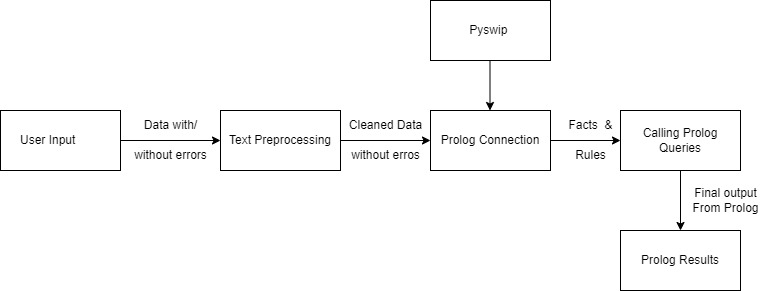
\includegraphics[width=15cm, height = 8cm]{Images/Architecture.jpg}
    \caption{Overall Architecture}
    \label{fig:Overall Architecture}
\end{figure}

To develop a domain-specific interface, we are going to use adequate knowledge representations of entities in the system.\cite{rohil2018natural} First order logic programming construct will be used in developing this knowledge base. Our system will implement the schema for the domain-specific language known as "entity network". Every schema entry is represented in the form of "Entity Association Entity" conveying that, the two entities are confined together by the given "Association".\cite{baeldungFirstOrderLogic} An example of the above statement would be "magnetism of a symbol." The knowledge base developed will have an organised and structured Prolog predicates, i.e facts and rules. The facts consist of elements and several properties of the periodic table. The rules about the periodic table will be represented using the schema of relations. A Python-based console application\cite{pypi} acting as an interface between the Prolog knowledge base and the user, has been implemented as shown in the sections below.

\subsection{Python}

Artificial Intelligence projects are different from traditional software projects. The difference lies in the technology stack, the skills required for AI-based projects, and the need for in-depth research. For
implementing AI projects we need to use a programming language that is stable, flexible, and easy to integrate with other software. Python provides all of these, as it is a high-level, interpreted, and general-purpose programming language. It is easy to learn, understand and implement when compared to other programming languages. It is also dynamically typed and garbage collected.\cite{pythonWelcomePythonorg} Python contains so many built-in libraries for Machine Learning and Natural Language Processing. Currently, in all the IT industries, Machine Learning Engineers are mostly using Python for AI and NLP-related projects as it is very flexible and easy to implement.    

\subsection{Natural Language Processing}

The ability of a machine to read, comprehend and derive a possible meaning from human languages is known as Natural Language Processing. NLP tends to process large volumes of textual data at ease. It also allows for Structuring a highly unstructured data source.\cite{ibmWhatNatural} At present, there are numerous open source libraries for NLP which help us to perform operations easily. We have also leveraged the use of NLP libraries for our implementation in Python. In this project, we have used the NLTK library in python for Natural Language Processing.


\subsection{Prolog}

A simple logic programming language, widely used in the field of Artificial Intelligence. It was predominantly used as a declarative programming language. The core of Prolog lies in the logic that is being applied.\cite{swiprologManual} Logic is expressed as relations called Facts and Rules. It is easy to build a data representation and does not require much programming effort. In this project, we have created facts and rules for the Periodic Table. Execution of a Prolog program is initiated by the user's posting of a single goal, called the query.\\
\newline
Sample Prolog facts and rules are shown below.\\
\newline
\textbf{Sample Facts for Periodic Table Group}\\
\newline
period\_group(1,'H',hydrogen,1,1,cavendish).\\
period\_group(2,'He',helium,18,1,janssen).\\
period\_group(3,'Li',lithium,1,2,arfvedson).\\
period\_group(4,'Be',beryllium,2,2,vaulquelin).\\
period\_group(5,'B',boron,13,2,gay-lussac).\\
period\_group(6,'C',carbon,14,2,prehistoric).\\
period\_group(7,'N',nitrogen,15,2,rutherford).\\
\newline
\textbf{Sample Facts for Physical Properties}\\
\newline
physical(1,'H',hydrogen,null,yes,0.0000899,14.175,20.28,0.79,2.2).\\
physical(2,'He',helium,null,yes,0.000179,null,4.22,0.49,null).\\
physical(3,'Li',lithium,yes,null,0.534,453.85,1615,2.1,0.98).\\
physical(4,'Be',beryllium,yes,null,1.85,1560.15,2742,1.4,1.57).\\
physical(5,'B',boron,null,null,2.34,2573.15,4200,1.2,2.04).\\
physical(6,'C',carbon,null,yes,2.27,3948.15,4300,0.91,2.55).\\
physical(7,'N',nitrogen,null,yes,0.00125,63.29,77.36,0.75,3.04).\\
\newline
\textbf{Sample Facts for Magnetic Properties}\\
\newline
type(1,'H',hydrogen,nonmetal).\\
type(2,'He',helium,noble\_gas).\\
type(3,'Li',lithium,alkali\_metal).\\
type(4,'Be',beryllium,alkaline\_earth\_metal).\\
type(5,'B',boron,metalloid).\\
type(6,'C',carbon,nonmetal).\\
type(7,'N',nitrogen,nonmetal).\\
\newline
\textbf{Sample Facts for Element Types}\\
\newline
type(1,'H',hydrogen,nonmetal).\\
type(2,'He',helium,noble\_gas).\\
type(3,'Li',lithium,alkali\_metal).\\
type(4,'Be',beryllium,alkaline\_earth\_metal).\\
type(5,'B',boron,metalloid).\\
type(6,'C',carbon,nonmetal).\\
type(7,'N',nitrogen,nonmetal).\\
\newline
\textbf{Sample Facts for Element Phases}\\
\newline
type(1,'H',hydrogen,nonmetal).\\
type(2,'He',helium,noble\_gas).\\
type(3,'Li',lithium,alkali\_metal).\\
type(4,'Be',beryllium,alkaline\_earth\_metal).\\
type(5,'B',boron,metalloid).\\
type(6,'C',carbon,nonmetal).\\
type(7,'N',nitrogen,nonmetal).\\
\newline
\textbf{Sample Rules for Periodic Table Group}\\
\newline
elements\_in\_a\_group(Group,Symbol,Element):-period\_group(\_,Symbol,Element,Group,\_,\_).\\
atomic\_number(Symbol,Element,Number):-period\_group(Number,Symbol,Element,\_,\_,\_).\\
name\_of(Symbol,Element):-period\_group(\_,Symbol,Element,\_,\_,\_).\\
discoverer(Element,Discoverer):-period\_group(\_,\_,Element,\_,\_,Discoverer).\\
metal\_or\_nonmetal(Element,Y):-physical(\_,\_,Element,Y,\_,\_,\_,\_,\_,\_).\\
density(Element,D):-physical(\_,\_,Element,\_,\_,D,\_,\_,\_,\_).\\




\subsection{Working}

\begin{enumerate}
    \item Obtain the user input as a string.
    \item Once the input is read, the program uses the NLTK libraries to pre-process the text. Stemming, lemmatization, emoji conversion, and stop words removal are all included in pre-processing.
    \item Cleaned, error-free data after pre-processing is received.
    \item The Pyswip module in Python, which links Python with Prolog, is used to feed this data as input to Prolog.
    \item Based on the user’s input its respective prolog rules and queries are called.
    \item Prolog returns the findings.
\end{enumerate}


%%%%%%%%%%%%%%%%%%%%%%%%%%%%%%%%%%%%%%%%%%%%%%%%
%%%%%%%%%%%%%%%%%%%%%%%%%%%%%%%%%%%%%%%%%%%%%%%%
\begin{figure}[htp]
    \centering
    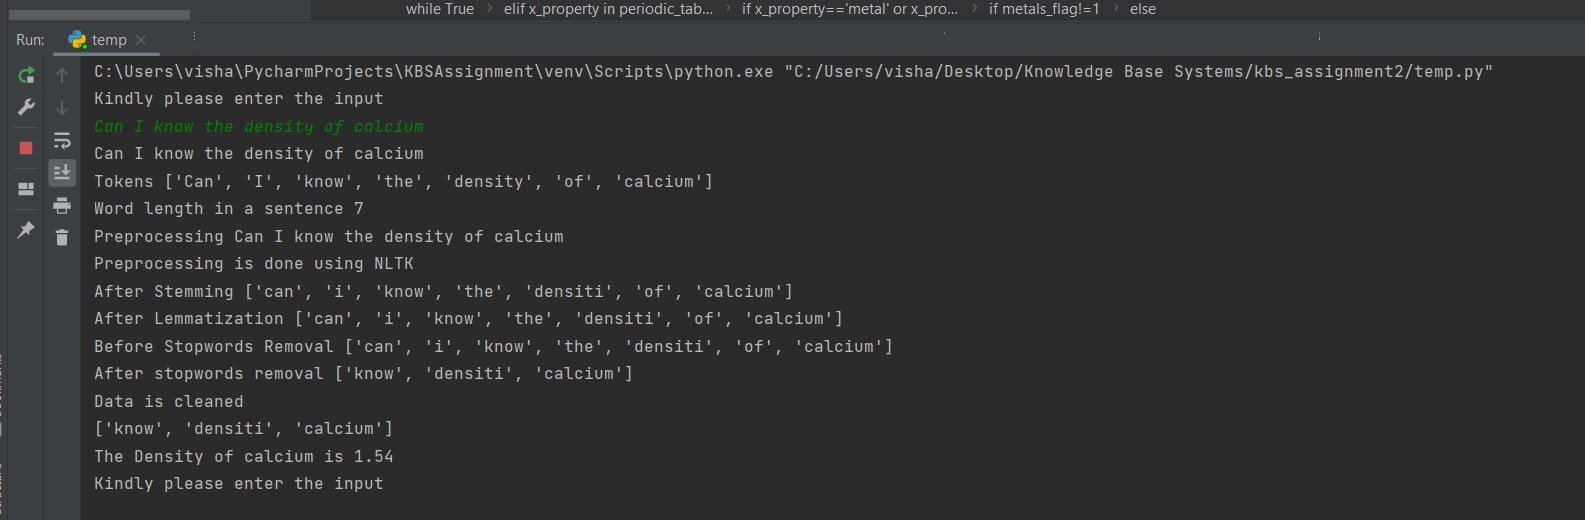
\includegraphics[width=15cm, height = 7cm]{Images/sc-1.jpg}
    \caption{User input without any errors}
    \label{fig:Example 1}
\end{figure}

\begin{figure}[htp]
    \centering
    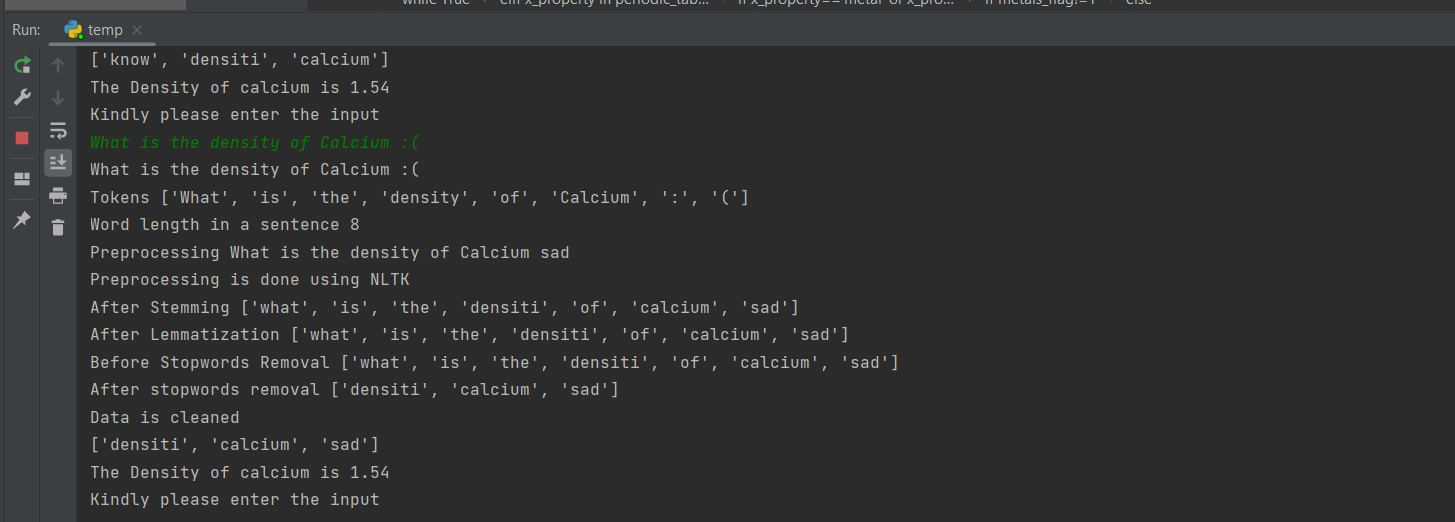
\includegraphics[width=15cm, height = 7cm]{Images/sc-2.jpg}
    \caption{User input with Emoji's}
    \label{fig:Example 2}
\end{figure}

\begin{figure}[htp]
    \centering
    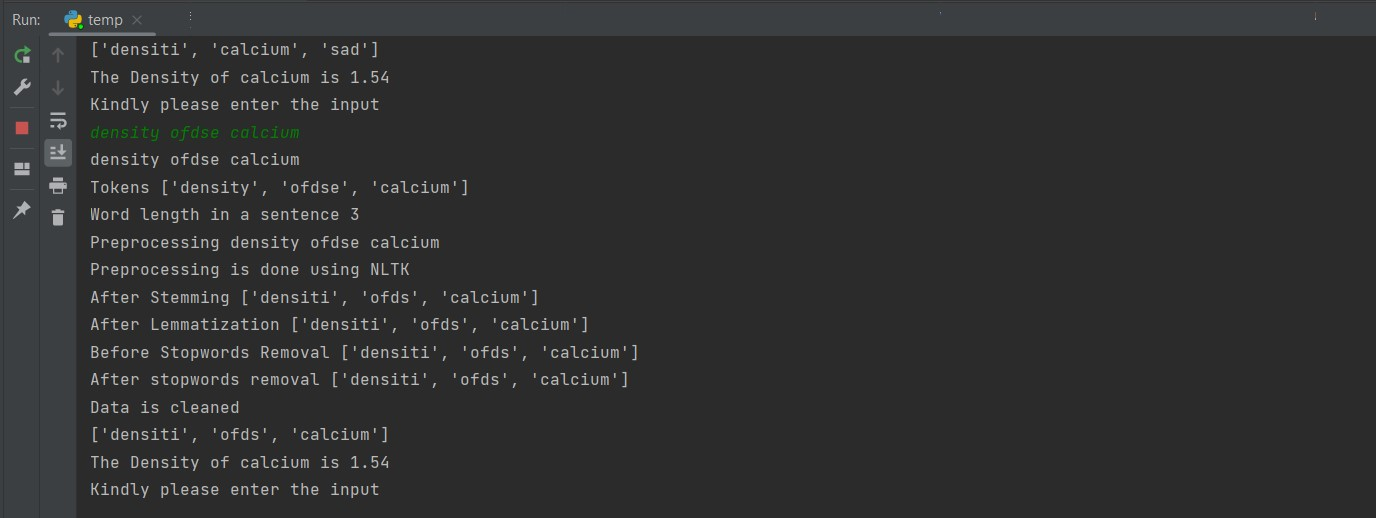
\includegraphics[width=15cm, height = 7cm]{Images/sc-3.jpg}
    \caption{User input with some errors}
    \label{fig:Example 3}
\end{figure}

\begin{figure}[htp]
    \centering
    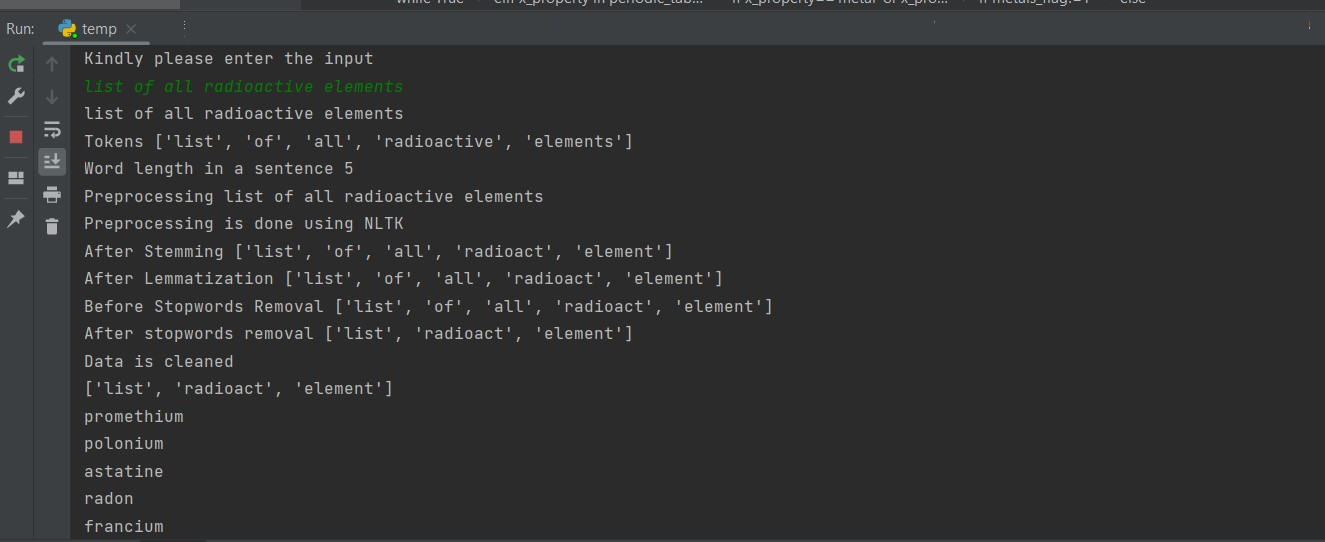
\includegraphics[width=15cm, height = 7cm]{Images/sc-4.jpg}
    \caption{Different type of Question and its response}
    \label{fig:Example 4}
\end{figure}

\begin{figure}[htp]
    \centering
    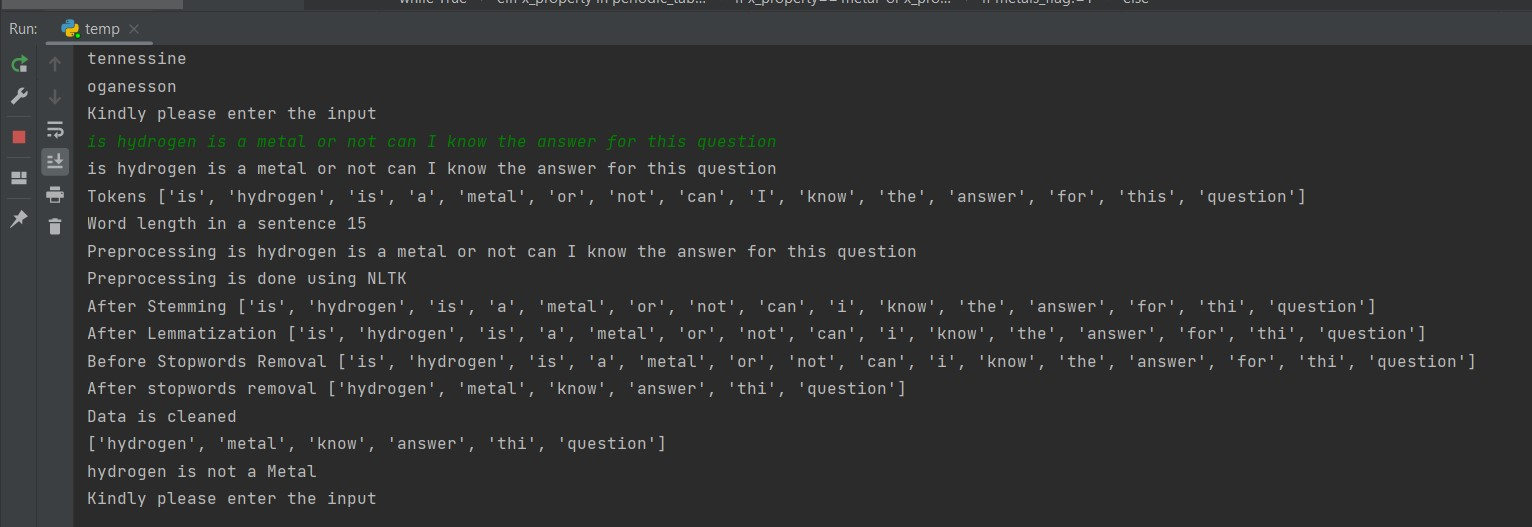
\includegraphics[width=15cm, height = 7cm]{Images/sc-5.jpg}
    \caption{Ground queries}
    \label{fig: Example 5}
\end{figure}

\begin{figure}[htp]
    \centering
    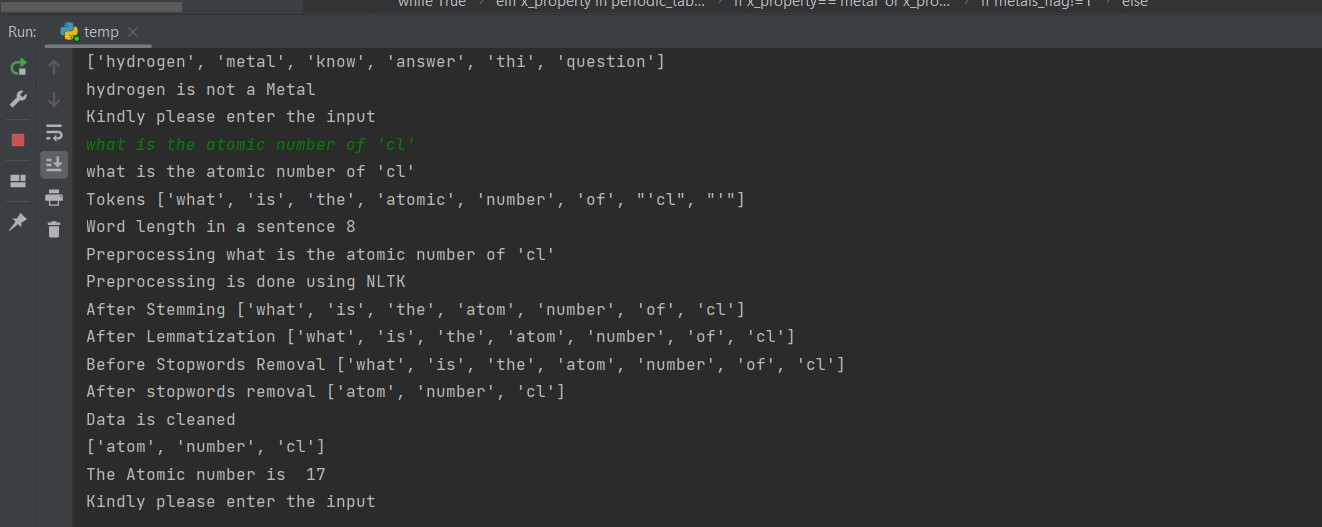
\includegraphics[width=15cm, height = 7cm]{Images/sc-6.jpg}
    \caption{Finding Atomic number of an Element}
    \label{fig: Example 6}
\end{figure}

\begin{figure}[htp]
    \centering
    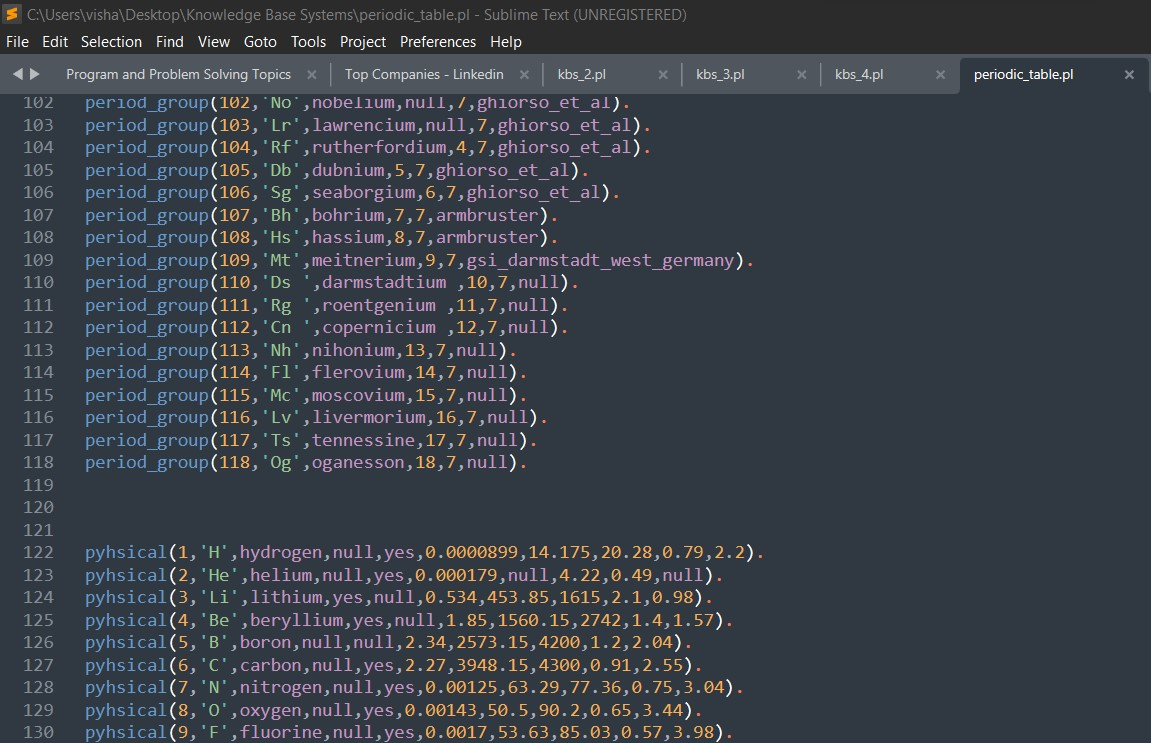
\includegraphics[width=15cm, height = 7cm]{Images/sc-10.jpg}
    \caption{Prolog Rules for Periodic Table}
    \label{fig: Example 7}
\end{figure}

\begin{figure}[htp]
    \centering
    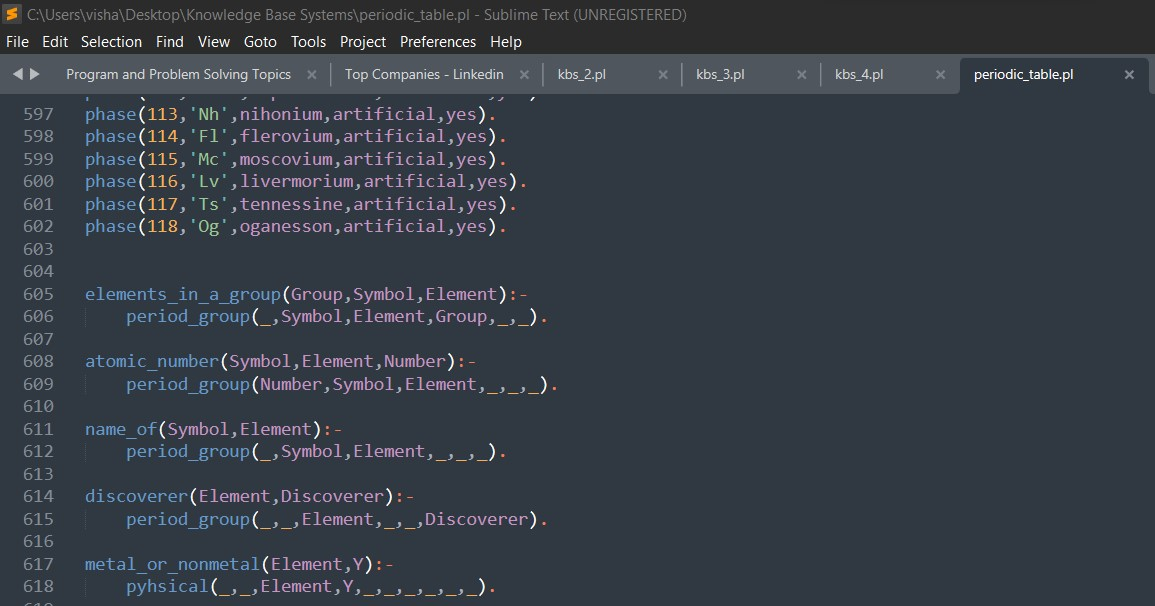
\includegraphics[width=15cm, height = 7cm]{Images/sc-7.jpg}
    \caption{Prolog Facts for Periodic Table}
    \label{fig: Example 8}
\end{figure}

\begin{figure}[htp]
    \centering
    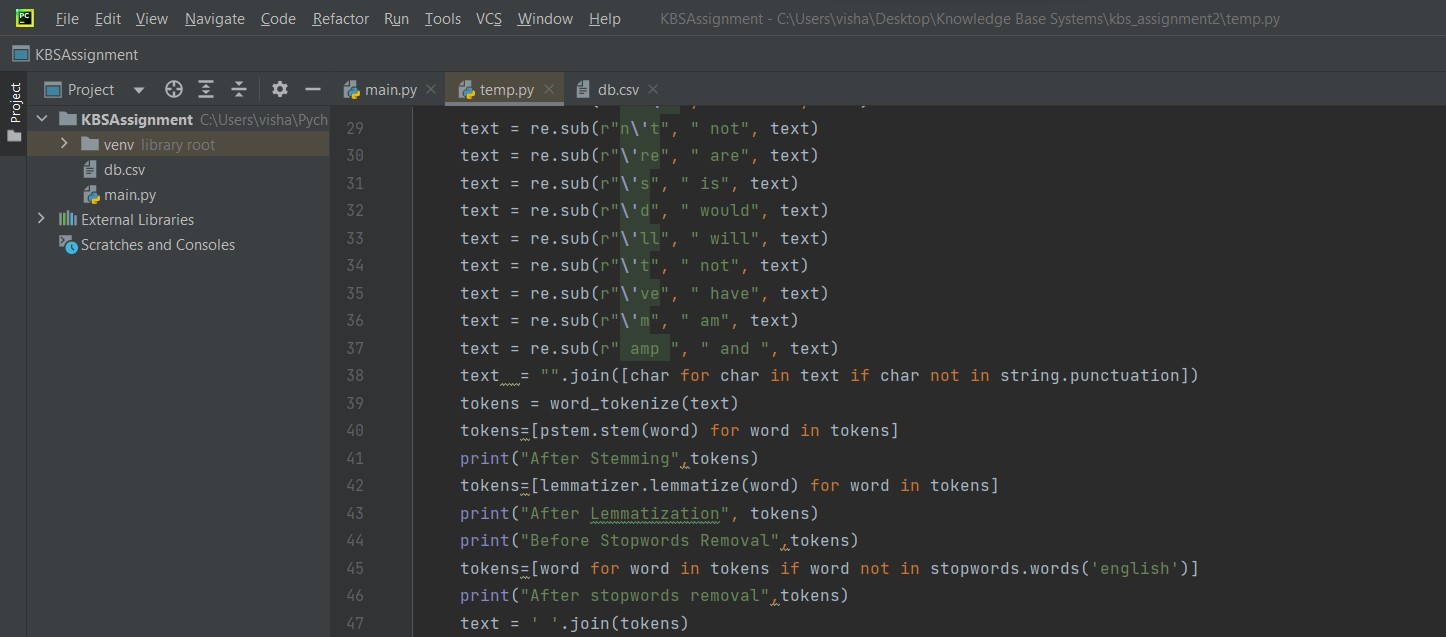
\includegraphics[width=15cm, height = 7cm]{Images/sc-8.jpg}
    \caption{NLP Preprocessing using NLTK}
    \label{fig: Example 9}
\end{figure}

\begin{figure}[htp]
    \centering
    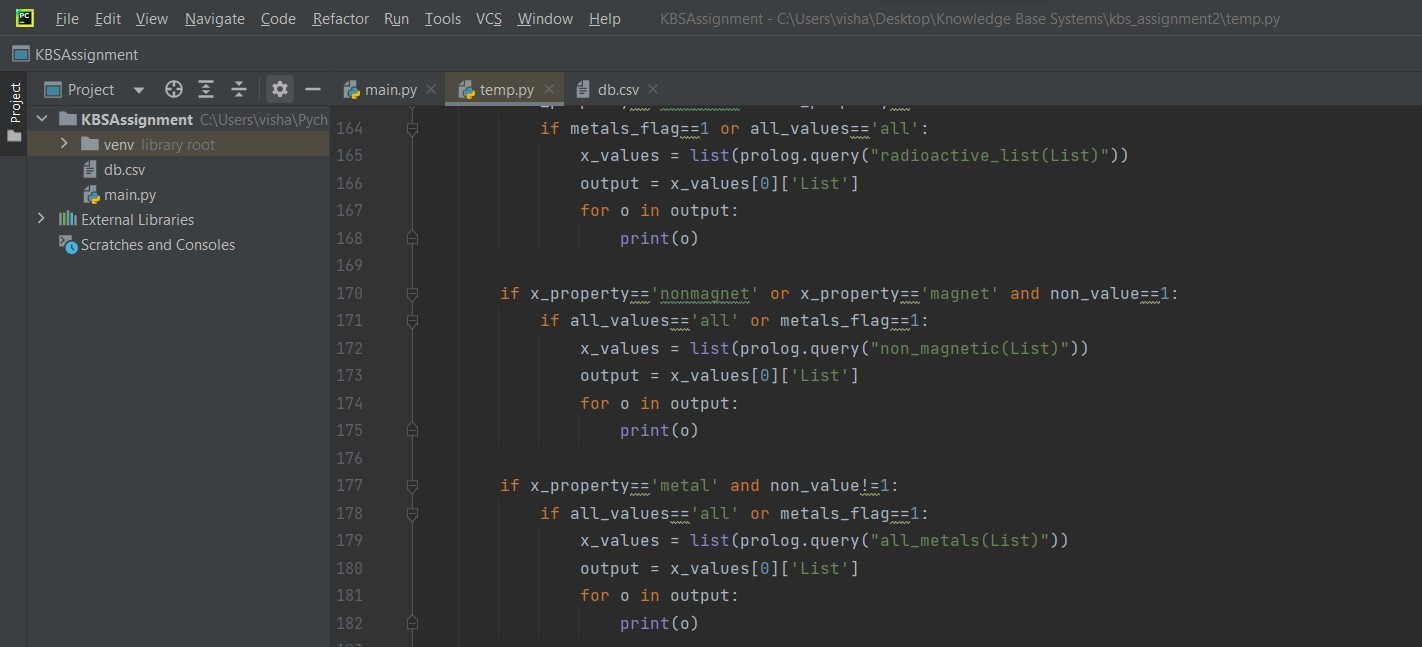
\includegraphics[width=15cm, height = 7cm]{Images/sc-9.jpg}
    \caption{Connecting Prolog and Python using Pyswip}
    \label{fig: Example 10}
\end{figure}


\newpage
%%%%%%%%%%%%%%%%%%%%%%%%%%%%%%%%%%%%%%%%%%%%%%%%
\section{Research Team}
%%%%%%%%%%%%%%%%%%%%%%%%%%%%%%%%%%%%%%%%%%%%%%%%
The roles and responsibilities of each team member have been displayed below.\\

\textbf{\textit{Ananya Varsha}}\\
Researched and web-scrapped periodic table data. Created entire knowledge base for the periodic table in Prolog. Assisted in the creation of code base for NLP in Python\\ 

\textbf{\textit{Saghana Mahesh Sarma}}\\
Researched on NLP and it's utilization on Python. Created a knowledge transfer article for the team on NLP. Assisted in the creation of Prolog Knowledge-base.\\

\textbf{\textit{Sivakumaran Malli Janardhanan}}\\
Web-scrapped entire periodic table data. Created all rules, procedures, queries for Prolog Knowledge base. Assisted in the integration of Python with Prolog.\\

\textbf{\textit{Vishanth Surresh}}\\
Integrated Python with Prolog. Developed code base for running Prolog code in python. Applied several NLP rules using pre-defined libraries. \\

%%%%%%%%%%%%%%%%%%%%%%%%%%%%%%%%%%%%%%%%%%%%%%%%
\section{Conclusion}
%%%%%%%%%%%%%%%%%%%%%%%%%%%%%%%%%%%%%%%%%%%%%%%%
In this course, we learnt how to work with Prolog and create numerous real-time knowledge base instances, how to create facts and rules, and accessing databases using Prolog. As Data Engineers/Scientists we wanted to connect Prolog with the latest technologies such as Artificial Intelligence and Machine Learning. So, integration between the logical programming of Prolog and the most widely utilized scripting language Python has been performed. It provided us with a wide array of learning experiences, both with Prolog and NLP.

%%%%%%%%%%%%%%%%%%%%%%%%%%%%%%%%%%%%%%%%%%%%%%%%
\section{Future Work}
%%%%%%%%%%%%%%%%%%%%%%%%%%%%%%%%%%%%%%%%%%%%%%%%
As per the current implementation, we have utilised dictionaries to identify the elements in the periodic table. For future work. we can train an NLP model to automatically detect the names of elements as soon as the user types. This reduces the threshold of storing additional hard-coded data and leverages the use of more powerful NLP concepts. 

\newpage
%%%%%%%%%%%%%%%%%%%%%%%%%%%%%%%%%%%%%%%%%%%%%%%%
\renewcommand{\refname}{References}
\bibliographystyle{plain}
\bibliography{References.bib}
%%%%%%%%%%%%%%%%%%%%%%%%%%%%%%%%%%%%%%%%%%%%%%%%
\end{document}
